\begin{figure}[H]
\centering
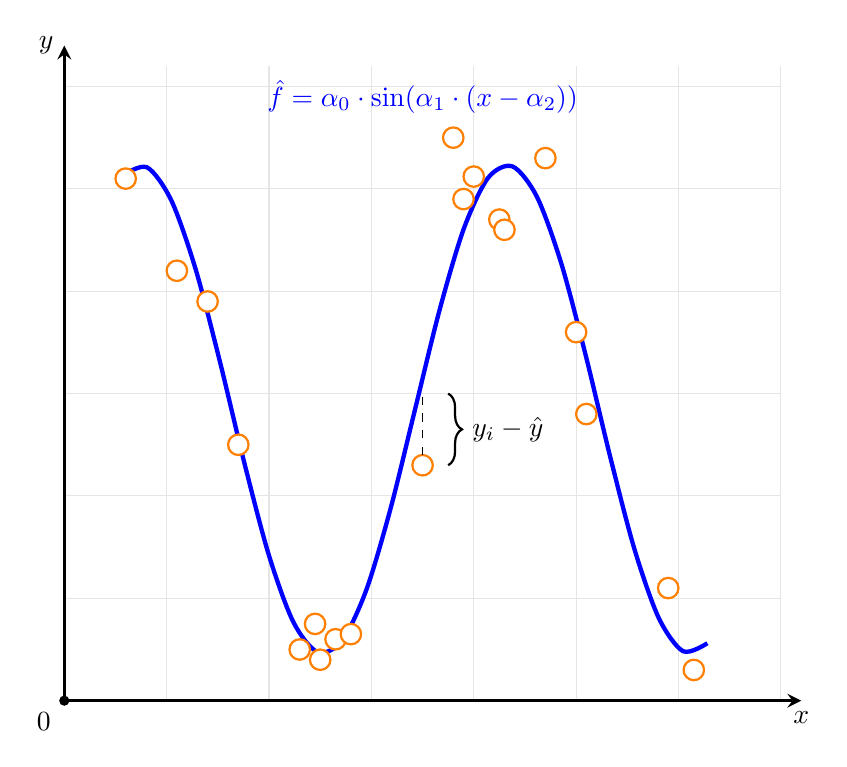
\begin{tikzpicture}[
	scale=1.3,
	axis/.style={
		-stealth,
		very thick
	}
]
% Gitter
\draw[gray!20] (0,0) grid (7,6.2);

% Achsen
\draw[axis] (0,0) -- (0,6.4) node[left]{$\boldsymbol{y}$};
\draw[axis] (0,0) -- (7.2,0) node[below]{$\boldsymbol{x}$};
\fill[black] (0,0) circle[radius=0.05];
\node at(-0.2,-0.2){$\boldsymbol{0}$};
    
    \begin{axis}[tick = none, axis lines=none]
    \addplot[smooth, color=blue, very thick] {sin(deg(x))}; 
    \end{axis}
    
    \node[blue] at(3.5,5.9){$\boldsymbol{\hat{f} = \alpha_0 \cdot \sin(\alpha_1 \cdot (x-\alpha_2))}$};
    
    \draw[orange,thick,fill=white] (1.1,4.2) circle[radius=0.1cm];
    \draw[orange,thick,fill=white] (0.6,5.1) circle[radius=0.1cm];
    \draw[orange,thick,fill=white] (1.4,3.9) circle[radius=0.1cm];
    \draw[orange,thick,fill=white] (1.7,2.5) circle[radius=0.1cm];
     \draw[orange,thick,fill=white] (2.3,0.5) circle[radius=0.1cm];
    \draw[orange,thick,fill=white] (2.45,0.75) circle[radius=0.1cm];
    \draw[orange,thick,fill=white] (2.65,0.6) circle[radius=0.1cm];
    \draw[orange,thick,fill=white] (2.8,0.65) circle[radius=0.1cm];
     \draw[orange,thick,fill=white] (2.5,0.4) circle[radius=0.1cm];
     
    \draw[orange,thick,fill=white] (4.25,4.7) circle[radius=0.1cm];
    \draw[orange,thick,fill=white] (4,5.12) circle[radius=0.1cm];
    \draw[orange,thick,fill=white] (4.7,5.3) circle[radius=0.1cm];
       \draw[orange,thick,fill=white] (3.8,5.5) circle[radius=0.1cm];
    \draw[orange,thick,fill=white] (4.3,4.6) circle[radius=0.1cm];
    \draw[orange,thick,fill=white] (3.9,4.9) circle[radius=0.1cm];
    
      \draw[orange,thick,fill=white] (5.1,2.8) circle[radius=0.1cm];
    \draw[orange,thick,fill=white] (5,3.6) circle[radius=0.1cm];
    \draw[orange,thick,fill=white] (5.9,1.1) circle[radius=0.1cm];
    \draw[orange,thick,fill=white] (6.15,0.3) circle[radius=0.1cm];
    
  \draw[orange,thick,fill=white] (3.5,2.3) circle[radius=0.1cm]; 
  \draw[dashed] (3.5,2.4) -- (3.5,3);   
    
    % Geschweifte Klammer
\draw[
	thick,
	black,
	decorate,
	decoration = {
		brace,
		amplitude = 5pt
	}
] (3.75,3) -- (3.75,2.3)
	node[
		midway,
		right,
		xshift = 5pt
] {$\boldsymbol{y_i -  \hat{y}}$};
\end{tikzpicture}
\caption[Grafische Darstellung der nichtlinearen Regression]{Grafische Darstellung der nichtlinearen Regression\protect\footnotemark}
\label{nlr}
\end{figure}
\footnotetext{Abbildung in Anlehnung an \textit{Günther} et al., Mathematische Modellbildung und Simulation, 2014, S. 86.}